\documentclass[conference]{IEEEtran}
\usepackage[T1]{fontenc}
\usepackage{cite}
\usepackage{amsmath,amssymb,amsfonts}
\usepackage{algorithmic}
\usepackage{graphicx}
\usepackage{textcomp}
\usepackage{seqsplit}
[]\def\BibTeX{{\rm B\kern-.05em{\sc i\kern-.025em b}\kern-.08em
    T\kern-.1667em\lower.7ex\hbox{E}\kern-.125emX}}
\begin{document}

\title{Volvo Cars' Automatic Brake System from a business perspective}

\author{\IEEEauthorblockN{1\textsuperscript{st} Emil Wihlander}
\IEEEauthorblockA{\textit{Computer science} \\
\textit{Faculty of Engineering, LTH}\\
Lund, Sweden \\
dat15ewi@student.lu.se}
\and
\IEEEauthorblockN{2\textsuperscript{nd} Jakob H\"{o}k}
\IEEEauthorblockA{\textit{Computer science} \\
\textit{Faculty of Engineering, LTH}\\
Lund, Sweden \\
dat15jh1@student.lu.se}
}

\maketitle

% ---------------------------------------------------------
% --------------------- Abstract  --------------------------
% ---------------------------------------------------------

\begin{abstract}
The paper describes and analyses Volvo Cars' automatic brake system called ``City Safety" from business, ethical and legal aspects. Given the development and progress of autonomous vehicles today it is interesting to analyse City Safety, which can be considered one of the first autonomous actions of a car. The analysis studies the system, first of all, from a business aspect where it discusses the financial driving forces, branding, patenting and open source software based on the three-layer product model and the cooperation with Zenuity. Secondly it debates City Safety's ethical concerns such as missed brake, incorrect brake and data collection with scenarios, both from a general perspective and from an individual perspective. Lastly, the article evaluates if City Safety is legal considering image capturing of the car's surroundings, the use of autonomous functions and the risk of unintended crashes. The analysis concludes that City Safety agrees with Volvo's business strategy and despite the ethical dilemmas it carries, the positives outweighs the negatives. The research of legal aspects was difficult to come by, but in the end Volvo seem to got all it's bases covered.
\end{abstract}

% ---------------------------------------------------------
% ------------------- Introduction  -----------------------
% ---------------------------------------------------------

\section{Introduction}
Autonomous vehicles (i.e.\ self-driving cars) are right around the corner with Volvo Cars aiming for a 2021 release to market. \cite{ADToMarket} Will it revolutionize the world or not? Who knows, what we do know is that the development had to start somewhere. One piece of the puzzle is to make the car have an automatic brake system. 

For example, imagine a car driving in the suburbs when suddenly a child accidentally kicks a ball onto the streets. The child makes a run for the ball, not aware of its surroundings. The driver brakes, but due to the reaction time of the driver the kid gets heavily injured. Now picture the same scenario with an automatic brake system. The car would be able to stop, by itself, in time and the accident would be avoided considering the car has (close to) no reaction time.Another possible scenario is that the driver crashes into the rear-end of the car in front due to inattention from using their phone or changing car settings or due to reduced sight from direct sunlight or harsh weather conditions.

An automatic brake system can, with it being always on, having close to no reaction time and using multiple sensors, potentially avoid, or at least mitigate, the hazardous situations presented above. With the driver being responsible for approximately 94\% of all car crashes, Volvo Cars, with its three key values, Environment, Quality and Safety, see great value in reducing those types of accidents. \cite{CrashStats,VolvoValues}

\subsection{Volvo Cars}
Volvo Cars has had a strong history of leading the industry when it comes to safety innovations with the three-point safety belt in 1959 and side impact protection, whiplash protection and roll-over protection in 1991, 1998 and 2002 respectively. 
While most of the innovation in the safety field up to the early -00 where protective features newer innovations focus on proactive safety such as the blind spot information system which was introduced in 2003. \cite{VolvoInnovation}

Volvo Cars has been offering an automatic brake system for rear-end collisions in its cars since 2008 and added a similar system for pedestrians in 2010. \cite{VolvoInnovation}
These functions has since their introduction been standard in all models and was in 2015, soon after the release of the second generation of ``City Safety'', rebranded so that all their different versions of automatic braking where included in their trademark ``City Safety''. \cite{CitySafety} With the announcement of the rebranding statistics proving the positive effect it has had on safety where provided and presented as a stepping stone towards autonomous vehicles. \cite{CitySafety}

\subsection{Zenuity}
In April 2017, a joint venture between Volvo Cars and Autoliv started its operations with the purpose to develop autonomous driving and advanced driver assist systems (ADAS). With both Autoliv and Volvo Cars licensing and transferring relevant intellectual property and moving personnel over to Zenuity the development of ADAS functions moved from in-house development to a separate unit. Zenuity's software will be sold to both third parties through Autoliv as well as Volvo Cars directly. \cite{ZenuityLaunch} Since automatic brake systems are classified as ADAS these where most likely included in the transfer from Volvo Cars to Zenuity.

\subsection{OSS}
Open source software (OSS) is a software open for anyone to read, modify and distribute. However, depending on the license of the OSS, tit might be more or less permissive. \cite{OSS}

\subsection{Software Patents}
Software patents are hard to grasp, from the beginning patents were meant as a legal protection for inventors. Patents could be viewed as a reward and acknowledgment of a scientist's success, dedication and time spent on an invention. The patent itself gave the inventor monopoly of the invention and therefore protects from potential thieves who steal the idea and use it for their own purpose. \cite{SoftwarePatent} At that time, the kind of inventions would typically be a physical product such as post-office drawer lock. \cite{LockPatent}

A software program usually implies a computer program. The definition of a computer program is several lines of instruction given to a computer which will execute them sequentially. One may not patent the lines of instructions, however, in conjunction with an executing computer it can be patentable. The reasoning is that a software program needs to be part of a process and in this case an executing computer is considered a process. In Europe, The European Patent Convention (EPC) has taken the ``process'' definition a step further. \cite{SoftwarePatent}
\begin{quotation}
``A computer program claimed by itself is not excluded from patentability if the program, when running on a computer or loaded into a computer, brings about, or is capable of bringing about, a technical effect which goes beyond the (normal' (sic) physical interactions between the program (software) and the computer (hardware) on which it is run." \cite[p. 36]{SoftwarePatent}
\end{quotation} 

To summarize, one cannot patent the software program code itself, but with some kind of hardware it is possible.
\subsection{Big Data}
Nowadays a company's big struggle is not to store all collected data, it is how to use it. The data is called ``Big Data''. \cite{ExploitBigData} Depending on the software, the collected data could be commute patterns, phone usage or as simple as the amount of user. With this kind of information, the company can make smart decisions. The downside is, the more data one got, the harder it is to process. To take fully advantage of the stored information the processing velocity is key. Another problem is the variety of data a company got. What information is in reality useful? \cite{SpeedDataEco} 

% ---------------------------------------------------------
% --------------Description of the system  ----------------
% ---------------------------------------------------------

\section{Description of the system}
The provided source describes the ``Collision Warning with Full Auto Brake and Pedestrian Detection'' system which is a complement to the first generation of ``City Safety''. The second generation (current) ``City Safety'' uses similar hardware, with the exception that the radar (and camera) is located at the top of the windscreen rather than in the grille, it will therefore be assumed that the systems are similar. \cite{SysDescription,RACam,DelphiVolvo}

The system consists of four main parts. The camera unit, the radar unit, the data fusion unit and a control unit for the automatic brake software. The control unit will communicate with the brake control unit, display control unit and sound control unit. The camera, radar and data fusion are all part of the unit, called ``RACam'', provided by Delphi. \cite{SysDescription,DelphiVolvo} No information was found that any open source software is used in the system.

\begin{figure}
	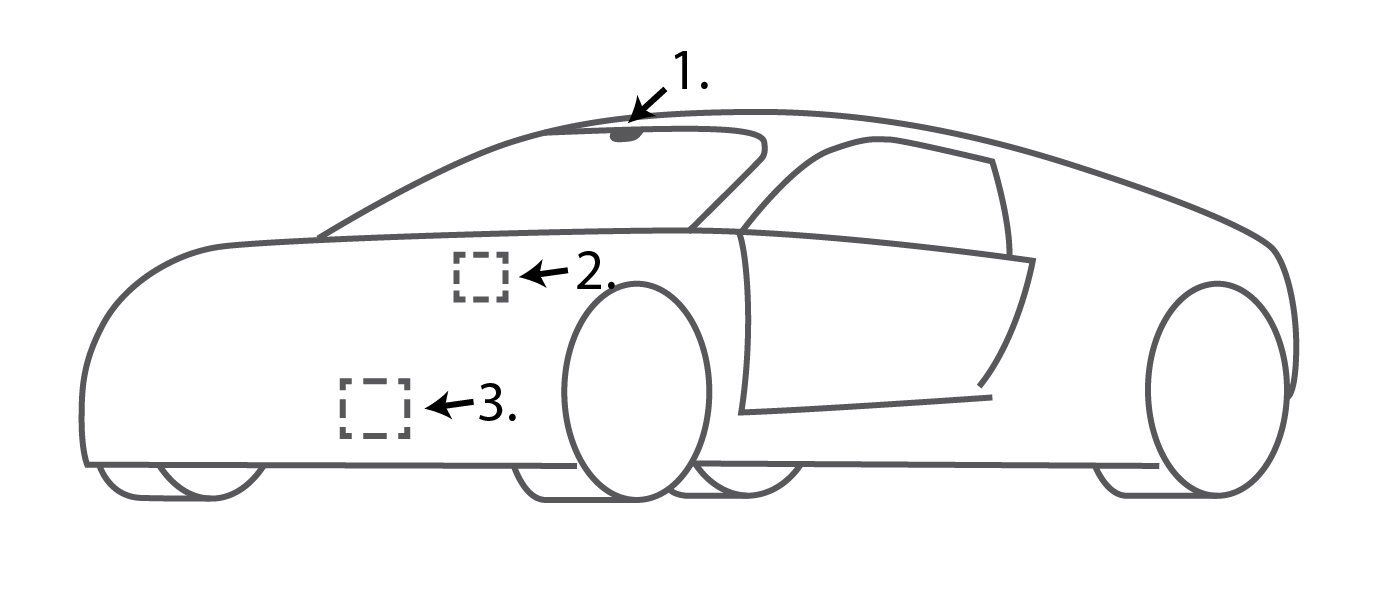
\includegraphics[scale=0.25]{overview.png}
	\caption{1. is the ``RaCam'', 2. is the display and sound control unit and 3. is the brake control unit. (The locations for all control units except the ``RaCam'' are guesses).}
\end{figure}

\subsection{RACam}
The data from the camera and radar are sent to the data fusion unit. The radar data is used for finding objects in front of the car and the distances to these objects. The camera image is used for classification of the found objects and therefore verifies whether they are vehicles, pedestrians, bicyclists or large animals. The unidentified objects are discarded\footnote{Which objects the ``RACam'' can identify depends which year model the car is.}. The data fusion helps reduce the risk of a false positive i.e. the car would brake without any real risks for collision. \cite{SysDescription}

\subsection{Control unit for automatic brake}
The control unit takes the calculations from the ``RACam'' and analyzes which objects are at risk of being hit based on their size, direction of movement and speed and the host car's speed and angle of the steering wheel. If an object is determined to be at risk a mathematical model is applied. If the model determines that the collision is imminent if the host car does not brake, the brakes are applied and the car will be able to stop if the relative speed is 60 km/h or less\footnote{The limitations are different depending on the type of object in front. \cite{CitySafetyDefinition}} with the latest version. \cite{SysDescription, CitySafetyDefinition}

If the mathematical model determines that the risk of a collision is likely it will notify the display and sound control unit to warn the user with an icon and sound. The user will hopefully brake before the automatic braking needs to be activated. \cite{CitySafetyDefinition}

% ---------------------------------------------------------
% ------------------- Business Aspects  -------------------
% ---------------------------------------------------------
\section{Business aspects}
City Safety does not generate any revenue as it is not sold as an upgrade, but is standard in all models. This begs the question, which are the financial driving forces behind City Safety? This will be analyzed from the perspective of the ``Three-layer product model'' presented in \cite{TeLESM}.

\subsection{Three-Layer product model}
One of the clear motivators during the initial development back in 2008 is, as presented before, its goal to be seen as the safest car brand. Volvo Cars' choice to release it as standard on all its models also seem to have the same motive. This positioned City Safety in the differentiating functionally layer but as the market has matured two thirds of all car models sold in the US have at least the option of adding city-speed emergency braking. Also, one of Volvo Cars' main competitors, Mercedes-Benz, have chosen to make automatic braking standard in most of its models.  \cite{AEBStatistics} This means that Volvo Car should start the process of moving the basic parts of City Safety from the differentiating functionality layer to the commoditized functionality layer. Thereby moving from optimizing for customer value to optimizing for the cost.

The automatic brake system is not OSS which mean the software is disclosed. This seems peculiar considering Volvo Cars' history of sharing safety features and moving them from differentiating to commoditized early on. This could imply two things, either Volvo Cars needs differentiation or they do not have the infrastructure (internal policies, standardization, servers for hosting, etc.) to do it.

\subsubsection{Differentiation}
When Volvo Cars back in the days shared the three-point safety belt it was easier to differentiate whereas today it is harder to separate one car brand from another, apart from design and trademark. Nowadays there are some ways to differentiate, e.g. price, reputation, specifications (top velocity, acceleration) or safety. This could be the reason why Volvo Cars is not making the automatic brake system OSS, to have some kind of uniqueness and to strengthen the brand's reputation, i.e. safety first. Despite the fact that the function is moving from differentiating to commoditized, it can still be seen as the former since it is a highly requested feature among consumers. \cite{AEBStatistics,VolvoVision}

Why is uniqueness of great importance? Let us take an example. If there were two jumpers in the same color, same price and same size, the only difference is the brand. Which jumper would one chose? In this case, the brand's reputation would be the only thing that mattered. Imagine the same example, but, the brand is the same and the price is different. Now the answer is more obvious, one would purchase the cheaper jumper. Now consider this, combine the two examples above. Two jumpers with same color and same size but with different brand and price. Harder decision has to be made, pay a higher price for a brand or pay less for another. Depends on the reputation, if the pricier jumper's company has a reputation of having better quality, the extra charge might be worth it. If we apply these examples to cars instead. Volvo Cars is trying to make the customer consider safety of the car rather than just performance or price. When a customer is considering the safety of the car, it is already a win but this how Volvo Cars can make a profit.

\subsubsection{Lacking infrastructure}
Making functions OSS is a great way to move a function to the commoditized functionality layer to reduce ownership cost but a  reasonable explanation why this has not happened is that Volvo Cars is not mature enough as a software company to release open source software. It is only recently automakers have moved to large scale software development as they are traditionally hardware makers. Software giants such as Microsoft, who have been in the software industry for over 30 years, have not had any major presence in the OSS community until recently which gives some sort of indication of the difficulties with moving to OSS. \cite{MicrosoftOSS}

In 2017 Volvo Cars announced a partnership with Google to use Android as the base operating system for the infotainment system\footnote{The infotainment system is the software running on the center stack display giving the user the ability to play music, change settings, get direction, etc.} in upcoming models. \cite{VolvoAndroid} This gives Volvo Cars, with minimal effort, the ability to build a light shell on top of a robust open source operating system instead of having the need to do this in house. As infotainment systems are more or less commodity this makes a resource intensive task, which does not add much customer value, a lot easier.

There are a lot of questions around how to handle liability, different sensors, modularity, etc. when it comes to open sourcing safety features since it can have severe consequences. But it is easy to draw parallels between the move to android and the possibility that Volvo Cars will move toward more OSS in the future as features become commodity and Volvo Cars, and the rest of the industry, mature as software companies.

\subsection{Patents}
No patent could be found of Volvo Cars' automatic brake system. This may imply multiple things. For starters, it might mean that it is hard to get a patent of such software system. The reason it is difficult to get the system approved is that it requires the software system to be a part of a piece of hardware. It is no easy task to fulfil this requirement. The software might be using hardware that is already patented or that there are no isolated hardware Volvo Cars can patent with the software. 

Another speculation of why Volvo Cars has no patent of the automatic brake system could be, once again, differentiation. One cannot stress enough the importance of being able to separate from its competitors. A patent will force the inventor to reveal the ``recipe'' and everyone can attempt to create the same product only using a different method. Volvo Cars does not want to share their ``secret sauce'' and therefore choose not to patent it. \cite{SoftwarePatent}

\subsection{Zenuity}
Zenuity positions itself somewhere between in house development and open source development since it shares resources between companies and wishes to distribute development and maintenance cost over multiple buyers. If Zenuity manages to obtain a large customer base the number of stakeholders will increase drastically and will simulate an OSS community.

The difference between Zenuity and OSS is that the hardware the software runs on is still regulated. This could avoid some of the problems with open sourcing safety features mentioned earlier. With Zenuity acting as an intermediate step between in house and open source development and being a pure software company it could be positioned very well to thrive in the current transformation the industry is experiencing.

\subsection{Summary}
At the moment, City Safety gives Volvo Cars its business value by boosting Volvo Cars' brand strength in safety but by releasing City Safety as open source Volvo Cars could gain greatly, reduced maintenance cost and reinforcement to its safety image. Nevertheless, it is also a risk because automatic braking may not be ready to go from being differentiating to commodity, or another reason could be that the industry might not be ready and a backlash could present itself if something would go wrong.

The creation of Zenuity seems to be a counter move to the digitalization and problems around shared innovation and patents. It could help Volvo Cars make an informed decision in problems as the one described in the last paragraph and to be able to share knowledge and advance research.

% ---------------------------------------------------------
% ------------------- Ethical Aspects  --------------------
% ---------------------------------------------------------

\section{Ethical aspects}
One of the major ethical concerns is the process of moving control from the driver to an algorithm due to the questions regarding liability. If City Safety would fail to brake in a situation where the driver expects it to work it could be argued that City Safety ultimately is the reason for the accident. This happened during an unofficial demonstration of the feature. \cite{CitySafetyFail} Volvo Cars tries to avoid these incidents by having a clear communication as to how City Safety should be used. Their support site states:

\begin{quotation}
	``City Safety must not be used as an excuse for the driver to change his/her driving style. If the driver solely relies on City Safety to do the braking, there might be a risk of a collision sooner or later.'' \cite{CitySafetyLegal}
\end{quotation}

Volvo has also designed City Safety in such a way that i should not engage until it is absolutely necessary and then brake hard. This will, by the driver, most likely be perceived as too late and as an unpleasant deceleration. This will most likely urge the driver not to use City Safety for convenience.

On the other end a possible error would be if City Safety would engage without an actual impending collision. With a car behind this could result in a collision rather than avoiding one. It is stated that the risk of this happening is at an ``acceptably low level'' \cite{SysDescription} but that still leaves room for accidents.

These two scenarios together could put City Safety, and there by Volvo Cars, in ethically muddy waters. However, if you take into consideration the positive effect it has had on the number of rear-end collisions \cite{CitySafety} the positives vastly outweigh the negatives.

\subsection{Data Collection}

Data collection is nothing illegal as long as the user agrees to the terms. However, ethical speaking, one can argue if it should be allowed in the first place. A company may collect data, both sensitive and non-sensitive, from a user in order to process and do various operations. How the data is processed and used depends on the company, it can be showing relevant ads or used to get nearest hospital. \cite{GoogleAds,GoogleNearby,GoogleUserData} Some data may be harmless, such as a record of a purchase made a year ago. Certain data is essential, for instance one's bank account with transaction history and account balance. There are always two sides of the same coin and hence there is data that is sensitive and can be used against an individual. When using Google's army of products, one give up a hefty amount of information. \cite{GoogleUserData} Suppose the information gets in the wrong hands, it can revealed which removes the purpose of privacy. It has happened and it can happen again. \cite{TheFappening,EdwardSnowden} 

Volvo is collecting several different kind of user data and vehicle data. Personal data collected are for instance contact and demographic information. \cite{PrivacyPolicy} Bare in mind, collecting data is nothing new and is required when a customer purchases a car in order to identify the owner and for various other reasons. The interesting information Volvo collects comes from what they call ``vehicle-recorded data", where one can find ``location data (the position of the vehicle in case of an accident, etc.)" and ``surroundings data (temperature outside the vehicle, images, etc.)". \cite{PrivacyPolicy} Even though no source could be found whether City Safety stores data for later use, one cannot exclude the possibility that City Safety collects, for example, images of the car's surroundings and transmit it to a main server. It is likely that the images, by default, are not sent elsewhere but can be accessed with proper setup. Nonetheless, a costumer may find it disturbing that there's a possibility of being monitored, not only the car's location, but also the car's surroundings.

Despite the clear ethical dilemma any digital company faces regarding sensitive data, there are pros as well. One is the reassurance in case of accident, where Volvo or local authorities can access the drivers location and immediately can take action. Imagine a single-vehicle accident where the driver is unconscious and cannot call an ambulance, in this instance the location data collection is a saving grace. To allow City Safety to prevent accidents, which is another benefit, it is essential to capture images of the car's surroundings. Volvo evidently claims the data is in safe hands and will not be used in any manner that may harm the user or without the customers consent. \cite{PrivacyPolicy} With this in mind, one could say that the customer trades (somewhat) his/her privacy for increased safety. Still, considering the safety potential, it immensely compensates for the ethical dilemma of data collection.

\subsection{Future}
The current implementation uses a mathematical model for decision-making but the possibility that future versions would be designed with machine learning, or more specifically deep learning, is probable. Automakers have lately seen the benefits deep learning could provide in the development of ADAS and autonomous driving technologies. This has manifested itself through the launch of NVIDIA Drive PX and the multiple partners involved (e.g. Volvo, Tesla and Mercedes-Benz). \cite{DrivePX} Machine learning requires big and versatile data sets which would give Volvo Cars an incentive to collect user data to specifically improve the functionality.

% ---------------------------------------------------------
% ------------------- Legal Aspects  ----------------------
% ---------------------------------------------------------

\section{Legal aspects}
Many questions regarding ethical liability concerning user data and different driving scenarios were the system malfunctions arise, as presented in the last section. When it comes to the legal aspects the same questions remain.

No source could be found that can verify whether Volvo's automatic brake system is collecting data to a central server or not. As mentioned before, it is quite likely that, currently, the system is not distributing the gathered images to an entity outside of the car. No Internet connection is built in by default which strengthens previous statement. \cite{SensusConnect} However, in the future, there is a great chance that Volvo will store and utilize the gathered data.

Data collection links to Big Data, which might be essential for City Safety in the future. As mentioned, with Big Data smart decisions can be made, but collecting data such as the cars position and the video recording of its surroundings disrupt the privacy\footnote{As can be seen in figure 1 and 7 in \cite{SysDescription}.}. Wherever the chauffeur drives, someone can be watching and take advantage of the geographical position. The owner should be aware of this when purchasing, so in a way, it is his/her own choice of potentially being monitored. What if it is never disclaimed at purchase? The clueless person who is acquiring a car does not know that his/her position is observed. According to Volvo's privacy policy: ``...we will obtain your consent prior to collecting or using your Personal data. The request for your consent will be clear and specific..." which means Volvo will never collect or use one's personal data without a clear request. \cite{PrivacyPolicy} Unfortunately, the request in question could not be found, it is therefore not possible to evaluate how ``clear and specific" this request is. It is not far fetched that the request may be one long text of legal text where, honestly, almost no one reads through and just accepts. Nonetheless, if the user agrees to the agreement, the data collection is legal.

City Safety requires a video feed of the cars surroundings, which the pedestrians may be unaware of. They did not get the opportunity of choosing whether they wanted to be observed by cars or not. At least the buyer of the car chooses, hopefully aware, of having his/her position tracked. Surprisingly this is not illegal unless recording military vehicle or a prohibited area. \textbf{add source}

If City Safety missed a critical brake, who will be responsible? According to the disclaimer on Volvo's website it is always the driver's responsibility and should never, deliberately, wait for City Safety to activate. \cite{CitySafetyLegal}

National law has not adapted to the current changes that has happened to the automotive industry when it comes to ADAS systems. For example, in Sweden the driver is ultimately responsible under current law but during a system malfunction where the system actively causes an accident it could be argued that the manufacture would be responsible. \cite{LegalSweden}

% ---------------------------------------------------------
% ------------------- Summary  --------------------------
% ---------------------------------------------------------

\section{Summary}
The automatic brake system is part of several sections of Volvo Cars' strategy. It aligns with their image as a car brand the puts safety first as well as the whole industry's move towards automation and software development.

This product certainly makes sense from a business perspective but opens questions regarding how the development should be carried out and if the industry has managed to adopt to the current move to large-scale software development. The function also opens up for some concerns regarding ethical aspects but the positives outweighs the negatives. It seems as though national law has not adapted to the current shift the industry is experiencing and there is ambiguity that needs to be addressed.

The rise of proactive safety functions seem to continue but as long as ethical aspects are taken into account and legal aspects are discussed further these kind of functions will both contribute to Volvo Cars' business, and the general public, in a positive way.
% ---------------------------------------------------------
% ------------------- References  -------------------------
% ---------------------------------------------------------

\begin{thebibliography}{00}
	\bibitem{ADToMarket} 
	Volvo Car Corporation,
	`Autonomous Driving'',
	2017.
	[online]. Available: \seqsplit{https://www.volvocars.com/intl/about/our-innovation-brands/intellisafe/autonomous-driving}.
	[Accessed 12 Nov. 2017].
	
	\bibitem{CrashStats} 
	NHTSA,
	``Critical Reasons for Crashes Investigated in the National Motor Vehicle Crash Causation Survey'',
	2015.
	[online]. Available: \seqsplit{https://crashstats.nhtsa.dot.gov/Api/Public/ViewPublication/812115}.
	[Accessed 12 Nov. 2017].
	
	\bibitem{VolvoValues} 
	Volvo Car Corporation,
	``Company'',
	2017.
	[online]. Available: 
	\seqsplit{https://group.volvocars.com/company}.
	[Accessed 12 Nov. 2017].
	
	\bibitem{VolvoInnovation} 
	Volvo Car Corporation,
	``A heritage of innovation'',
	2017.
	[online]. Available: \seqsplit{https://www.volvocars.com/intl/about/our-company/heritage/innovations}.
	[Accessed 12 Nov. 2017].
	
	\bibitem{CitySafety} 
	Volvo Car Group,
	``Volvo Cars' standard safety technology cuts accident claims by 28 per cent'',
	2015.
	[online]. Available: \seqsplit{https://www.media.volvocars.com/global/en-gb/media/pressreleases/163733/volvo-cars-standard-safety-technology-cuts-accident-claims-by-28-per-cent}.
	[Accessed 13 Nov. 2017].
	
	\bibitem{ZenuityLaunch} 
	Autoliv,
	``Autoliv and Volvo Cars autonomous driving joint venture Zenuity starts operations'',
	2017.
	[online]. Available: \seqsplit{http://news.cision.com/autoliv/r/autoliv-and-volvo-cars-autonomous-driving-joint-venture-zenuity-starts-operations,c2240525}.
	[Accessed 14 Nov. 2017].
	
	\bibitem{OSS} 
	M. Henley and R. Kemp,
	``Open Source Software: An Introduction'', 
	Computer Law \& Security Report,
	vol. 24, pp. 77-85, 
	2008.
	
	\bibitem{SoftwarePatent} 
	A. Wilk,
	``Patentability of Software'',
	in 2012 IEEE International Conference on Software Science, Technology and Engineering,
	Herzlia, Israel,
	pp. 30-39,
	2012.
	
	\bibitem{LockPatent} 
	L. Yale,
	``Linus Yale'',
	31,278,
	1861.
	
	\bibitem{ExploitBigData} 
	J. Heidrich, A. Trendowicz and C. Ebert,
	``Exploiting Big Data's Benefit'',
	IEEE Software 
	vol. 33, no. 4, pp. 111-116,
	2016.
	
	\bibitem{SpeedDataEco} 
	J. Bosch,
	``Speed, data, and ecosystems: the future of software engineering'',
	IEEE Software,
	vol. 33, no. 1, pp. 82-88, 
	2016.
	
	\bibitem{SysDescription} 
	E. Coelingh, A. Eidehall and M. Bengtsson,
	``Collision Warning with Full Auto Brake and Pedestrian Detection - a practical example of Automatic Emergency Braking'',
	in 13th International IEEE Conference on Intelligent Transportation Systems, 
	Funchal, Portugal,
	pp. 155 - 160,
	2010.
	
	\bibitem{RACam} 
	Delphi,
	``Delphi Integrated Radar and Camera System'',
	2017.
	[online]. Available: \seqsplit{https://www.delphi.com/manufacturers/auto/safety/active/racam/}.
	[Accessed 22 Nov. 2017].
	
	\bibitem{DelphiVolvo} 
	Delphi,
	``Delphi First to Market with Integrated Radar and Camera System on Volvo Cars'',
	2014.
	[Online]. Available: \seqsplit{http://news.cision.com/market-engineering/r/delphi-first-to-market-with-integrated-radar-and-camera-system-on-volvo-cars,c9654815}.
	[Accessed 19 Dec. 2017].
	
	\bibitem{CitySafetyDefinition}
	Volvo Cars Support,
	``Parameters and subfunctions for City Safety'',
	2017.
	[Online]. Available: 
	\seqsplit{https://support.volvocars.com/uk/cars/pages/owners-manual.aspx?mc=v542\&my=2018\&sw=17w46\&article=bd3160158449cb66c0a8015159b3a7b8}.
	[Accessed 12 Dec. 2017].
	
	\bibitem{TeLESM} 
	H. Holmstr\"{o}m Olsson and J. Bosch,
	``From ad hoc to strategic ecosystem management: the `Three-Layer Ecosystem Strategy Model' (TeLESM)'',
	Journal of Software: Evolution and Process,
	vol. 29, no. 7, 
	2017.
	
	\bibitem{AEBStatistics}
	S. Sinclair,
	``Automatic Emergency Braking Availability Expands with 2017 Cars'',
	\emph{Consumer reports},
	2017.
	[Online]. Available:
	\seqsplit{https://www.consumerreports.org/car-safety/automatic-emergency-braking-availability-expands-with-2017-cars/}.
	[Accessed 19 Dec. 2017].
	
	\bibitem{VolvoVision} 
	Volvo Car Group,
	``Vision'',
	2017.
	[Online]. Available: 
	\seqsplit{https://group.volvocars.com/company/vision}. 
	[Accessed 22 Nov. 2017].
	
	\bibitem{MicrosoftOSS}
	S. Bhartiya,
	``How Microsoft Is Shifting Focus to Open Source'',
	2017.
	[online]. Available:
	\seqsplit{https://thenewstack.io/microsoft-shifting-emphasis-open-source/}.
	[Accessed 10 Jan. 2018].
	
	\bibitem{VolvoAndroid}
	Volvo Car Group,
	``Volvo Cars partners with Google to build Android into next generation connected cars'',
	2017.
	[Online]. Available:
	\seqsplit{https://www.media.volvocars.com/global/en-gb/media/pressreleases/208072/volvo-cars-partners-with-google-to-build-android-into-next-generation-connected-cars}.
	[Accessed 20 Dec. 2017].
	
	\bibitem{CitySafetyFail}
	V. Cruz Cid,
	``Volvo auto brake system fail'',
	2015.
	[Online]. Available:
	\seqsplit{https://www.youtube.com/watch?v=\_47utWAoupo}.
	[Accessed 21 Dec. 2017].
	
	\bibitem{CitySafetyLegal}
	Volvo Cars Support,
	``City Safety'',
	2017.
	[Online]. Available: \seqsplit{https://support.volvocars.com/uk/cars/pages/owners-manual.aspx?mc=y555\&my=2018\&sw=17w17\&article=f11aa8c30d28b105c0a801e8005b64ab}.
	[Accessed 12 Dec. 2017].
	
	\bibitem{GoogleAds}
	Google, 
	``Google Privacy | Why data protection matters'',
	2017.
	[Online]. Available:
	\seqsplit{https://privacy.google.com/how-ads-work.html}.
	[Accessed 15 Dec. 2017].
	
	\bibitem{GoogleNearby}
	Google,
	``Search and find nearby places'',
	2017.
	[Online]. Available: \seqsplit{https://support.google.com/maps/answer/4610185?co=GENIE.Platform\%3DAndroid\&hl=en}.
	[Accessed 15 Dec. 2017].
	
	\bibitem{GoogleUserData} 
	Google,
	``Google Privacy | Why data protection matters'',
	2017.
	[Online]. Available:
	\seqsplit{https://privacy.google.com/your-data.html}.
	[Accessed 15 Dec. 2017].
	
	\bibitem{TheFappening}
	C. Arthur,
	``Naked celebrity hack: security experts focus on iCloud backup theory'',
	\emph{the Guardian},
	2017.
	[Online]. Available: \seqsplit{https://www.theguardian.com/technology/2014/sep/01/naked-celebrity-hack-icloud-backup-jennifer-lawrence.}.
	[Accessed 15 Dec. 2017].
	
	\bibitem{EdwardSnowden}
	G. Greenwald, E. MacAskill and L. Poitras,
	``Edward Snowden: the whistleblower behind the NSA surveillance revelations'',
	\emph{the Guardian},
	2017.
	[Online]. Available: \seqsplit{https://www.theguardian.com/world/2013/jun/09/edward-snowden-nsa-whistleblower-surveillance.}.
	[Accessed 15 Dec. 2017].
	
	\bibitem{PrivacyPolicy}
	Volvo Cars Support,
	``CUSTOMER PRIVACY POLICY'',
	2017.
	[Online]. Available:
	\seqsplit{https://support.volvocars.com/uk/pages/article.aspx?article=58bd8ef320c39971c0a801513f4e18ef}.
	[Accessed 06 Dec. 2017].
	
	\bibitem{DrivePX}
	NVIDIA,
	``NVIDIA Drive PX'',
	2017.
	[Online]. Available:
	\seqsplit{https://www.nvidia.com/en-us/self-driving-cars/drive-px/}.
	[Accessed 21 Dec. 2017].
	
	\bibitem{SensusConnect}
	Volvo Cars Support,
	``Sensus Connect'',
	2017.
	[Online]. Available: \seqsplit{https://support.volvocars.com/uk/Pages/article.aspx?article=2f87dc53ab618edec0a801517aec401a}.
	[Accessed 06 Dec. 2017].
	
	\bibitem{LegalSweden}
	Riksdagen,
	"Sj\"alvk\"orande fordon p\r{a} v\"ag",
	2018.
	[Online]. Available:
	\seqsplit{https://www.riksdagen.se/sv/dokument-lagar/dokument/kommittedirektiv/sjalvkorande-fordon-pa-vag\_H3B1114}.
	[Accessed 07 Jan. 2018]
\end{thebibliography}

\newpage
\appendix
\section*{Contribution statement}
The introduction until the first subsection where written in collaboration.
\subsection{Emil}
\begin{itemize}
	\item
	The subsections Volvo Cars and Zenuity of  the Introduction.
	\item
	All of the Description of the system.
	\item
	Business aspects from beginning until the paragraph beginning with ``The automatic brake system is not OSS''.
	\item
	The subsections Lacking infrastructure, Zenuity and Summary of Business aspects.
	\item
	All of Ethical aspects except ``Data Collection".
	\item
	First and last paragraph of Legal aspects.
	\item
	All of Summary.
\end{itemize}
\subsection{Jakob}
\begin{itemize}
	\item
	All of Abstract
	\item
	The subsections OSS, Software Patents and Big data of the Introduction.
	\item
	The paragraph beginning with ``The automatic brake system is not OSS'' and the subsections Differentiation and Patents of Business aspects.
	\item
	``Data Collection" in Ethical aspects.
	\item
	Almost all of Legal aspects.
\end{itemize}

\end{document}
